\documentclass[]{article}
\usepackage{amsmath,amssymb}
\usepackage{graphicx}

\usepackage[utf8]{inputenc}
\usepackage[T1]{fontenc}
\usepackage[russian]{babel}


\usepackage{xcolor}
\usepackage{hyperref}
%\usepackage{autonum}
\renewcommand{\[}{\begin{equation}}
\renewcommand{\]}{\end{equation}}

%opening
\title{О непереполненном базисе скалярных и смешанных произведений сигма-матриц}
\author{Олег Лычковский, Филипп Усков}

\begin{document}

\maketitle

\begin{abstract}
	
\show \TeX
Исследуется вопрос о полном вращательно-инвариантном операторном базисе для спиновых систем. Получен полный непереполненный базис, и исследованы его простейшие свойства.

\end{abstract}

%%%%%%%%%%%%%%%%%%%%%%%%%%%%%%%%%%%%%%%%%%%%%%%%%%%%%%%%%%%%%%%%%%%%
%%%%%%%%%%%%%%%%%%%%%%%%%%%%%%%%%%%%%%%%%%%%%%%%%%%%%%%%%%%%%%%%%%%%
%%%%%%%%%%%%%%%%%%%%%%%%%%%%%%%%%%%%%%%%%%%%%%%%%%%%%%%%%%%%%%%%%%%%
\section{Введение}

В физике важную роль играют системы спинов $1/2$ с изотропным Гейзенберговским взаимодействием. Общий вид гамильтониана имеет вид:
\[
H=-\sum_{i\neq j}J_{ij}\vec\sigma_i\vec\sigma_j 
\label{k1}
\]
где $\vec\sigma_i = \{\sigma_i^x,\sigma_i^y,\sigma_i^z\}$ - вектор матриц Паули, $J_{ij}$ - константы связи, $i,j$ - нумеруют спины.

Состояние такой систмемы описаывается матрицей плотности $\rho$.
Поскольку гамильотониан изотропен, то матрица плотности тоже изотропна, и может быть разложена в базис:
\[A_i=\{ 1,  \;\;({\vec \sigma}_j{\vec\sigma}_k), \;\;
({\vec \sigma}_j{\vec\sigma}_k)({\vec \sigma}_l{\vec\sigma}_m)\;\;,\;\;...\}
\label{k2}
\]
Он конструируется из единичной матрицы и всевозможных скалярных и смешанных произведений сигма-матриц. 
Если мы требуем инвариантности матрицы плотности относительно обращений по времени, то в этом базисе будут только скалярные произведения (и единица),
а если не требуем, то благодаря тождеству 
\[
(\vec\sigma_1,\vec\sigma_2,\vec\sigma_3)
(\vec\sigma_4,\vec\sigma_5,\vec\sigma_6)= 
\begin{vmatrix}
	(\vec\sigma_1,\vec\sigma_4) & 	(\vec\sigma_1,\vec\sigma_5) & (\vec\sigma_1,\vec\sigma_6) \\
	(\vec\sigma_2,\vec\sigma_4) & 	(\vec\sigma_2,\vec\sigma_5) & (\vec\sigma_2,\vec\sigma_6) \\
	(\vec\sigma_3,\vec\sigma_4) & 	(\vec\sigma_3,\vec\sigma_5) & (\vec\sigma_3,\vec\sigma_6) \\
\end{vmatrix}
\label{k3}
\]
в каждом слагаемом ожно оставить не более одного смешанного произведения.

Матрица плотности, разложенная по такому базису, используется в частности при квадратичной параметризации \cite{kvadro},
для нахождения вариационного ограничения снизу энергии основного состояния \cite{variational}, 
а также для решения уравнения шредингера в виде $ H\rho = E\rho $ [???].
Также такой базис используется для нахождения интегралов движения гейзенберговской спиновой цепочки \cite{basisF}.

Недостатком такого базиса является его переполненность.
В настоящей статье опираясь на результаты работы \cite{sourceArticle}
мы построим полный но непереполненный базис изотропной системы.

%%%%%%%%%%%%%%%%%%%%%%%%%%%%%%%%%%%%%%%%%%%%%%%%%%%%%%%%%%%%%%%%%%%%
%%%%%%%%%%%%%%%%%%%%%%%%%%%%%%%%%%%%%%%%%%%%%%%%%%%%%%%%%%%%%%%%%%%%
%%%%%%%%%%%%%%%%%%%%%%%%%%%%%%%%%%%%%%%%%%%%%%%%%%%%%%%%%%%%%%%%%%%%
%\section{Цель и ход работы}
%Мы захотели получить этот базис в непереполненном виде, чтобы немного сократить объем вычилений.

%Мы нашли статью \cite{basis_f} про "базис f", но через год, когда мы ее всё-таки прочитали, оказалось что это вообще не имеет ни какого отношения к нашему базису.

%Мы решили посчитать сколько же на самом деле линейнонезависимых векторов в нашем базисе для небольшого числа спинов,
%нашли эту последовательность на OEIS, 
%и нашли статью, которая описывает, как строить непереполненный базис, и вот что там говориться:

%%%%%%%%%%%%%%%%%%%%%%%%%%%%%%%%%%%%%%%%%%%%%%%%%%%%%%%%%%%%%%%%%%%%
%%%%%%%%%%%%%%%%%%%%%%%%%%%%%%%%%%%%%%%%%%%%%%%%%%%%%%%%%%%%%%%%%%%%
%%%%%%%%%%%%%%%%%%%%%%%%%%%%%%%%%%%%%%%%%%%%%%%%%%%%%%%%%%%%%%%%%%%%
\section{Построение непереполненного базиса \cite{sourceArticle}}
Элементы базиса будем называть табличками. Эти таблички заполняются номерами спинов.

Столбец высоты 3 мы интерпретируем как смешанное произведение.
\[
\begin{tabular}{ | l | }
\hline
1 \\ \hline
2 \\ \hline
3 \\
\hline
\end{tabular} = (\vec \sigma_1, \vec \sigma_2, \vec \sigma_3) 
\label{k4}
\]
Пару столбцов мы интерпретируем как определитель скалярных произведений (или, что то же самое, обобщенный символ Кронекера\cite{kronecker_wiki}, свёрнутый со всеми векторами сигма-матриц).
\[
\begin{tabular}{ |l|l| }
\hline
1 & 4 \\ \hline
2 & 5\\ 
\hline
\end{tabular}
 =
 \sigma_1^{\alpha_1} \sigma_2^{\alpha_2} 
 (\delta_{\alpha_1\alpha_2}^{\alpha_4\alpha_5})
 \sigma_4^{\alpha_4} \sigma_5^{\alpha_5} 
 =
\begin{vmatrix}
(\vec\sigma_1,\vec\sigma_4) & (\vec\sigma_1,\vec\sigma_5)\\
(\vec\sigma_2,\vec\sigma_4) & (\vec\sigma_2,\vec\sigma_5)\\
\end{vmatrix}
\label{k5}
\]
например

пара столбцов длины 1 это просто скалярное произведение
\[
\begin{tabular}{ |l|l| }
\hline
1 & 2 \\
\hline
\end{tabular}
= (\vec \sigma_1, \vec \sigma_2)
\label{k6}
\]
пара столбцов длины 3 равна произведению двух смешанных произведений (каждое соответствует  своему столбцу)
\[
\begin{tabular}{ |l|l| }
\hline
1 & 4 \\ \hline
2 & 5\\ \hline
3 & 6\\
\hline
\end{tabular}
= 
\begin{vmatrix}
(\vec\sigma_1,\vec\sigma_4) & (\vec\sigma_1,\vec\sigma_5) & (\vec\sigma_1,\vec\sigma_6) \\
(\vec\sigma_2,\vec\sigma_4) & (\vec\sigma_2,\vec\sigma_5) & (\vec\sigma_2,\vec\sigma_6) \\
(\vec\sigma_3,\vec\sigma_4) & (\vec\sigma_3,\vec\sigma_5) & (\vec\sigma_3,\vec\sigma_6) \\
\end{vmatrix}
=
(\vec \sigma_1, \vec \sigma_2, \vec \sigma_3)
(\vec \sigma_4, \vec \sigma_5, \vec \sigma_6)
\label{k7}
\]

В базис войдут элементы, удовлетворяющие следующим критериям:
\begin{itemize}
	\item кажда строка в табличке содержит число ячеек не больше чем в предыдущей строке
	\item строк не больше 3
	\item Для четного числа спинов:
	\begin{itemize}
		\item столбцы разбиваются на пары, высоты столбцов в каждой паре совпадают
	\end{itemize}
	\item Для нечетного числа спинов:
	\begin{itemize}
		\item в начале таблички добавляется столбец высоты 3
		\item оставшиеся N-3 ячейки делаем как для четного числа
	\end{itemize}
	Примеры форм табличек:
	
	\begin{tabular}{ |l|l| }
		\hline
		количество спинов &  Примеры форм табличек\\ 
		\hline
		2 & 
			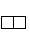
\includegraphics{1x2.png}
		\\ \hline
		3 &
		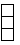
\includegraphics{3x1.png}
		\\ \hline
		4 & 
		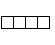
\includegraphics{1x4.png}
		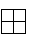
\includegraphics{2x2.png}
		\\ \hline
		5 &
		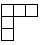
\includegraphics{3x3.png}
		\\ \hline
		6 &
		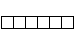
\includegraphics{1x6.png}
		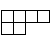
\includegraphics{2x4.png}
		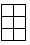
\includegraphics{3x2.png}
		\\ \hline
		7 &
		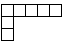
\includegraphics{3x5.png}
		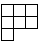
\includegraphics{3x3(7).png}
		\\ \hline
		8 &
		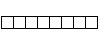
\includegraphics{1x8.png}
		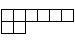
\includegraphics{2x6.png}
		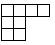
\includegraphics{3x4.png}
		\\ \hline
	\end{tabular}
		
	\item после чего заполняем эти таблички различающимися номерами спинов так, чтобы каждая строка и каждый столбец был отсортирован по возрастанию номера спина (при необходимости спины можно перенумеровать в любой последовательности)
	
	Примеры заполнения одной таблички:
\[
\begin{tabular}{ |l|l|l|l| }
\hline
1 & 2 \\ \hline
3 & 4 \\ \hline
5 & 6 \\
\hline
\end{tabular}
	\quad	
\begin{tabular}{ |l|l|l|l| }
\hline
1&2 \\ \hline
3&5 \\ \hline
4&6 \\
\hline
\end{tabular}
	\quad	
\begin{tabular}{ |l|l|l|l| }
\hline
1&3 \\ \hline
2&4 \\ \hline
5&6 \\
\hline
\end{tabular}
	\quad	
\begin{tabular}{ |l|l|l|l| }
\hline
1&3 \\ \hline
2&5 \\ \hline
4&6 \\
\hline
\end{tabular}
	\quad	
\begin{tabular}{ |l|l|l|l| }
\hline
1&4 \\ \hline
2&5 \\ \hline
3&6 \\
\hline
\end{tabular}
\label{k8}
\]
\end{itemize}

Пример всего базиса для 4 спинов:
\[
\begin{tabular}{ |l|l|l|l| }
\hline
1 & 2 & 3 & 4 \\ 
\hline
\end{tabular}
\quad	
\begin{tabular}{ |l|l| }
\hline
1 & 2 \\ \hline
3 & 4 \\
\hline
\end{tabular}
\quad	
\begin{tabular}{ |l|l| }
\hline
1 & 3 \\ \hline
2 & 4 \\
\hline
\end{tabular}
\quad	
\label{example4}
\]

Была написана функция \cite{basis_gen_code}, которая генерирует все возможные элементы базиса, и их число совпало с формулой из статьи\cite{sourceArticle}
\[
Q_n = \sum_{r=0}^{[n/2]}\frac{n!(3r-n+1)}{(n-2r)!r!(r+1)!}.
\label{k9}
\]
Ранее нами была обнаружена гипотеза, что пара столбцов длины 4 равна 0, и что этим объясняются все линейные зависимости в базисе с четным числом спинов.
\[
\begin{tabular}{ |l|l| }
\hline
1 & 5 \\ \hline
2 & 6\\ \hline
3 & 7\\ \hline
4 & 8\\
\hline
\end{tabular}
= 
\begin{vmatrix}
(\vec\sigma_1,\vec\sigma_5) & (\vec\sigma_1,\vec\sigma_6) & (\vec\sigma_1,\vec\sigma_7) & (\vec\sigma_1,\vec\sigma_8)\\
(\vec\sigma_2,\vec\sigma_5) & (\vec\sigma_2,\vec\sigma_6) & (\vec\sigma_2,\vec\sigma_7) & (\vec\sigma_2,\vec\sigma_8)\\
(\vec\sigma_3,\vec\sigma_5) & (\vec\sigma_3,\vec\sigma_6) & (\vec\sigma_3,\vec\sigma_7) & (\vec\sigma_3,\vec\sigma_8)\\
(\vec\sigma_4,\vec\sigma_5) & (\vec\sigma_4,\vec\sigma_6) & (\vec\sigma_4,\vec\sigma_7) & (\vec\sigma_4,\vec\sigma_8)\\
\end{vmatrix}
=0 .
\label{k10}
\]
Был замечен факт, что если для четного числа спинов сгененрировать все возможные таблички без ограничения числа строк,
то их общее число оказалось равно количеству элементов нашего исходного переполненного базиса
\[
N_n=\begin{cases}
\frac{n!}{2^{n/2}(n/2)!} & (n=2k)\\
\frac{n!}{3\dot 2^{(n-1)/2}((n-3)/2)!} & (n=2k+1)
\end{cases}
\label{k11}
\]
откуда можно сформулировать гипотезу, что скорее всего все таблички, у которых число строк больше 4 (они =0), дают все линейные зависимости в исходном базисе.
Для нечетного количества спинов аналогичный факт нами пока не придуман.

Можно сравнить размеры базисов переполненного и непереполненного:

\begin{tabular}{ |l|l l l l l l l l l l l| }
	\hline
	$n$   & 2 & 3 & 4 & 5  & 6  & 7   & 8   & 9    & 10  & 15    & 20    
	\\ \hline
	$N_n$ & 1 & 1 & 3 & 10 & 15 & 105 & 105 & 1260 & 945 & 4.7E6 & 6.5E8 
	\\ %\hline
	$Q_n$ & 1 & 1 & 3 & 6  & 15 & 36  & 91  & 232  & 603 & 83097 & 1.3E7 
	\\ \hline
\end{tabular}

\begin{tabular}{ |l|l l l l l l l l| }
	\hline
	$n$   & 10  & 20    & 30     & 40     & 50     & 60     & 70     & 80
	\\ \hline
	$N_n$ & 945 & 6.5E8 & 6.2E15 & 3.2E23 & 5.8E31 & 2.9E40 & 3.4E49 & 8.0E58
	\\ %\hline
	$Q_n$ & 603 & 1.3E7 & 4.4E11 & 1.7E16 & 7.2E20 & 3.3E25 & 1.5E30 & 7.4E34
	\\ \hline
\end{tabular}

\section{Заключительное замечание}
Количество элементов в полученном базисе меньше,
однако чтобы использовать в уравнении Шрёдингера $H \rho = E \rho$, нужно еще научиться умножать элементы нашего базиса (из $\rho$) на скалярные произведения (из $H$), и полученный результат вновь раскладывать по базису.
Для переполненного базиса это было реализовано ранее (и описано в предыдущих статьях \cite{variational}.
Для нового непереполненного базиса это сделать пока не удалось (так чтобы при этом не переходить к старому переполненному базису, что сводит на нет преимущества нового непереполненного базиса).

\begin{thebibliography}{3}
	\bibitem{sourceArticle}
	D. L. Andrews and T. Thirunamachandran, On three-dimensional rotational averages, {\it J. Chem. Phys.,} {\bf 67 (1977),} 5026-5033.
	\href{https://oeis.org/A005043/a005043_1.pdf}
	{https://oeis.org/A005043/a005043\_1.pdf}
	
	\bibitem{kvadro} N. Il'in, E. Shpagina, F. Uskov, O. Lychkovskiy, 
	Squaring parametrization of constrained and unconstrained sets of quantum states, {\it J. Phys. A: Math. Theor.} {\bf 51, 085301} (2018)
	\href{https://arxiv.org/abs/1704.03861}{https://arxiv.org/abs/1704.03861}
	
	\bibitem{variational}
	F. Uskov, O. Lychkovskiy. A variational lower bound on the ground state of a many-body system and
	the squaring parametrization of density matrices {\it// J. Phys.: Conf. Ser.} {\bf 1163, 012057} (2019).
	\href{https://arxiv.org/abs/1902.09246}{https://arxiv.org/abs/1902.09246}
	
	%\bibitem{Anderson} Anderson PW 1951
	%Limits on the energy of the antiferromagnetic Ground State
	%{\it Phys. Rev.} {\bf 83(6)} 1260
	
	\bibitem{basis_gen_code}
	\href{https://github.com/FeelUsM/ScalarMixedSpins/blob/master/tables.nb}
	{https://github.com/FeelUsM/ScalarMixedSpins/blob/master/tables.nb}
	
	\bibitem{basisF}
	P. Grabowski and Pierre Mathieu, Quantum Integrals of Motion for the Heisenberg Spin Chain, {\it  Modern Physics Letters A} {\bf 9.24 (1994): 2197-2206.}
	\href{https://arxiv.org/abs/hep-th/9403149}{https://arxiv.org/abs/hep-th/9403149}
	
	\bibitem{kronecker_wiki}
	\href{https://en.wikipedia.org/wiki/Kronecker_delta#Generalizations}
	{https://en.wikipedia.org/wiki/Kronecker\_delta\#Generalizations}
	
\end{thebibliography}

\end{document}
